% This template was originally by R. Jacob Vogelstein
% Updated on March 1, 2010 by Noah J. Cowan
% Updated on May 18, 2014 by Brian Weitzner at https://github.com/weitzner/jhu-thesis-template
% Updated on January 29, 2016 by John Muschelli at https://github.com/muschellij2/PhD_Thesis
% Updated on April 13, 2016 by Leonardo Collado Torres and available at https://github.com/lcolladotor/jhu-thesis-template. View (read-only) at Overleaf here https://www.overleaf.com/read/tqdzgmrxgbtg
% Updated on May 7, 2019 by Bin Ren and available at https://github.com/seawander/jhu-thesis-template-astro

%% It's your responsability to make sure that your thesis complies with 
%% JHU's formatting rules available at http://guides.library.jhu.edu/etd/formatting

\documentclass[12pt]{report}

%% This was the setup recommended at https://github.com/weitzner/jhu-thesis-template
% \documentclass[12pt,oneside,final]{thesis}

\pdfminorversion=4\relax
\pdfobjcompresslevel=0\relax
%% Followed the information from https://www.overleaf.com/latex/examples/creating-pdf-slash-a-and-pdf-slash-x-files/bbbycnbyqhnm#.Vw6_XBMrLm1 to create a PDF/A file in Overleaf
\usepackage[a-1b]{pdfx} % Need this to create a PDF/A file

\usepackage{pdfpages}
\usepackage{datetime}
%\usepackage{deluxetable}
\pagestyle{myheadings}
%\topmargin=0.25in
\topmargin=0.05in
\textheight=8.15in
\textwidth=5.6in
\oddsidemargin=0.7in
\raggedbottom
\newdimen \jot \jot=5mm
\brokenpenalty=10000
 

%\usepackage[utf8]{inputenc} % Seems to cause a conflict with fontenc and lmodern
%\DeclareUnicodeCharacter{00A0}{ }
\usepackage[T1]{fontenc}
\usepackage{lmodern} % load a font with all the characters
%\usepackage{hyperref}
\usepackage{tocbibind} % need this to contents adding for TOC
\usepackage{setspace}
\setstretch{1.05}
\usepackage{RJournal_nogeom} % Changes the colors of links among other things
%\usepackage[all]{hypcap}
\usepackage[hypcap=true]{caption}
\hypersetup{linktocpage}
\usepackage{amsmath,amssymb,array}
\usepackage{booktabs}
%\usepackage{subfig}
\usepackage{subcaption}
\usepackage{longtable}
\usepackage[final]{changes} % Enabling final revision of changes (added by Bin Ren). 
% You might have used \includepackages[trackchanges]{aastex62} in your manuscript, and the above package will reduce your burden of deleting the \added, \deleted, \replaced commands.



%% load any required packages here
\usepackage{graphicx}
\usepackage{float}
\usepackage{tikz}
\usepackage{graphics} 
\usetikzlibrary{positioning}
\usetikzlibrary{shapes,arrows}
\usepackage{dcolumn}
\usepackage{amsmath, amssymb, bm}
\usepackage{hyperref}
\usepackage{CJK} % Enabling simplified Chinese characters (added by Bin Ren)
\usepackage{float}
\usepackage{wrapfig}
\usepackage{pdflscape}
\usepackage{rotating}
\usepackage{tabularx}
\usepackage{adjustbox}
\usepackage{threeparttable}

\usepackage{booktabs}
%\usepackage[strings]{underscore}

\makeatletter
\newsavebox{\@tabnotebox}
\providecommand\tmark{} % so having ctable or not is irrelevant
\providecommand\tnote{}
\newenvironment{tabularwithnotes}[3][c]
  {\long\def\@tabnotes{#3}%
   \renewcommand\tmark[1][a]{\makebox[0pt][l]{\textsuperscript{\itshape##1}}}%
   \renewcommand\tnote[2][a]{\textsuperscript{\itshape##1}\,##2\par}
   \begin{lrbox}{\@tabnotebox}
   \begin{tabular}{#2}}
  {\end{tabular}\end{lrbox}%
   \parbox{\wd\@tabnotebox}{
     \usebox{\@tabnotebox}\par
     \smallskip\@tabnotes
   }%
  }
\makeatother

\input{astrodependencies.txt} % Translation of the short commands in ADS (added by Bin Ren)
 



\definecolor{cyan(process)}{rgb}{0.17, 0.18, 0.47}
\definecolor{green(colorblind)}{rgb}{0.0, 0.4, 0}



%%%%%%%%%%%%%%%%%%%%%%%%%%%%%%%%%%%%%%%%%%%%%%%%%%%%%%%%%%%%%%%%
% DOI from Segmentation
% Don't use - needs hyperref
%%%%%%%%%%%%%%%%%%%%%%%%%%%%%%%%%%%%%%%%%%%%%%%%%%%%%%%%%%%%%%%%
%\makeatletter
%\providecommand{\doi}[1]{%
%  \begingroup
%    \let\bibinfo\@secondoftwo
%    \urlstyle{rm}%
%    \href{http://dx.doi.org/#1}{%
%      doi:\discretionary{}{}{}%
%      \nolinkurl{#1}%
%    }%
%  \endgroup
%}
%\makeatother

%%%%%%%%%%%%%%%%%%%%%%%%%%%%%%%%%%%%%%%%%%%%%%%%%%%%%%%%%%%%%%%%
% StartKNITR STUFF -- added by John Muschelli
%%%%%%%%%%%%%%%%%%%%%%%%%%%%%%%%%%%%%%%%%%%%%%%%%%%%%%%%%%%%%%%%
\usepackage{color}
%% maxwidth is the original width if it is less than linewidth
%% otherwise use linewidth (to make sure the graphics do not exceed the margin)
\makeatletter
\def\maxwidth{ %
  \ifdim\Gin@nat@width>\linewidth
    \linewidth
  \else
    \Gin@nat@width
  \fi
}
\makeatother

\definecolor{fgcolor}{rgb}{0.345, 0.345, 0.345}
\newcommand{\hlnum}[1]{\textcolor[rgb]{0.686,0.059,0.569}{#1}}%
\newcommand{\hlstr}[1]{\textcolor[rgb]{0.192,0.494,0.8}{#1}}%
\newcommand{\hlcom}[1]{\textcolor[rgb]{0.678,0.584,0.686}{\textit{#1}}}%
\newcommand{\hlopt}[1]{\textcolor[rgb]{0,0,0}{#1}}%
\newcommand{\hlstd}[1]{\textcolor[rgb]{0.345,0.345,0.345}{#1}}%
\newcommand{\hlkwa}[1]{\textcolor[rgb]{0.161,0.373,0.58}{\textbf{#1}}}%
\newcommand{\hlkwb}[1]{\textcolor[rgb]{0.69,0.353,0.396}{#1}}%l
\newcommand{\hlkwc}[1]{\textcolor[rgb]{0.333,0.667,0.333}{#1}}%
\newcommand{\hlkwd}[1]{\textcolor[rgb]{0.737,0.353,0.396}{\textbf{#1}}}%

\usepackage{framed}
\makeatletter
\newenvironment{kframe}{%
 \def\at@end@of@kframe{}%
 \ifinner\ifhmode%
  \def\at@end@of@kframe{\end{minipage}}%
  \begin{minipage}{\columnwidth}%
 \fi\fi%
 \def\FrameCommand##1{\hskip\@totalleftmargin \hskip-\fboxsep
 \colorbox{shadecolor}{##1}\hskip-\fboxsep
     % There is no \\@totalrightmargin, so:
     \hskip-\linewidth \hskip-\@totalleftmargin \hskip\columnwidth}%
 \MakeFramed {\advance\hsize-\width
   \@totalleftmargin\z@ \linewidth\hsize
   \@setminipage}}%
 {\par\unskip\endMakeFramed%
 \at@end@of@kframe}
\makeatother

\definecolor{shadecolor}{rgb}{.97, .97, .97}
\definecolor{messagecolor}{rgb}{0, 0, 0}
\definecolor{warningcolor}{rgb}{1, 0, 1}
\definecolor{errorcolor}{rgb}{1, 0, 0}
\newenvironment{knitrout}{}{} % an empty environment to be redefined in TeX
\makeatletter
\newcommand\gobblepars{%
    \@ifnextchar\par%
        {\expandafter\gobblepars\@gobble}%
        {}}
\makeatother
%%%%%%%%%%%%%%%%%%%%%%%%%%%%%%%%%%%%%%%%%%%%%%%%%%%%%%%%%%%%%%%%
% End KNITR STUFF
%%%%%%%%%%%%%%%%%%%%%%%%%%%%%%%%%%%%%%%%%%%%%%%%%%%%%%%%%%%%%%%%


\usepackage[
style = authoryear, 
sorting = nyt, 
dashed = false,
maxbibnames = 99,
backend = bibtex,
natbib = true
]{biblatex}  % Sort the references in ApJ style (changed by Bin Ren)

% If you want to exclude some portions from the bibliography
\AtEveryBibitem{
\clearfield{note}
\clearfield{month}
}


\usepackage{enumerate}

%\tolerance=10000

%\makeglossary % enable the glossary
\graphicspath{{intro_chapter/}{chapter_apj/}{chapter_apj_dup/}} % change it accordingly!
% NOTE: If you have multiple folders/chapters, do NOT repeat the above line, but just add another "{}"  (added by Bin Ren)


\setcounter{tocdepth}{4}
\setcounter{secnumdepth}{4}
\begin{document}
\begin{CJK*}{UTF8}{gbsn} % Enabling simplified Chinese characters (added by Bin Ren)



%\newcommand{\bm}[1]{ \mbox{\boldmath $ #1 $} }
\newcommand{\bin}[2]{\left(\begin{array}{@{}c@{}} #1 \\ #2
             \end{array}\right) }
\renewcommand{\contentsname}{Table of Contents}
\baselineskip=24pt
 
\pagenumbering{roman}
\thispagestyle{empty}
\begin{center}
\vspace*{.25in}
{\bf\LARGE{Fancy Title of Your Thesis}}\\ % change it accordingly!
\vspace*{.75in}
{\bf by} \\*[18pt]
\vspace*{.2in}
{\bf First Last (姓名)}\\ % change it accordingly! 
% The above line is an example of simplified Chinese characters (added by Bin Ren)
\vspace*{1in}
{\bf A dissertation submitted to The Johns Hopkins University\\
in conformity with the requirements for the degree of\\
Doctor of Philosophy }\\
\vspace*{.75in}
{\bf Baltimore, Maryland} \\
{\bf \monthname, \the\year} \\     % change it accordingly! % Enabling simplified Chinese characerters (added by Bin Ren)
\vspace*{.5in}
\begin{small}
{\bf \copyright{ }\the\year\ by First Last (姓名)} \\ % change the year if needed!
{\bf All rights reserved}
\end{small}
\end{center}
\newpage 

% Add acknowledgements
\pagestyle{plain}
\pagenumbering{roman}
\setcounter{page}{2}
\chapter*{Abstract}

This is your abstract.

\vfill
\noindent Research Advisor: First1 Last1 \hfill \\
\noindent Academic Advisor: First2 Last2 \hfill
\chapter*{Thesis Committee}

\section*{}
\subsection*{Primary Readers}

\begin{singlespace}


\indent First1 Last1\\
\indent \indent  Astronomer\\
%\indent \indent Department of ChangeMe\\
\indent \indent  Space Telescope Science Institute \\


\smallskip 

\noindent First2 Last2\\
\indent \indent Assistant Professor\\
\indent \indent Department of Physics \& Astronomy\\
\indent \indent  Johns Hopkins Krieger School of Arts \& Sciences \\

\smallskip 

\noindent First3 Last3 \\
\indent \indent Associate Professor\\
\indent \indent Department of Physics \& Astronomy \\
\indent \indent  Johns Hopkins Krieger School of Arts \& Sciences \\

\smallskip


\noindent First4 Last4 \\
\indent \indent Professor\\
%\indent \indent Affiliation1, and\\
\indent \indent Department of Physics \& Astronomy \\
%\indent \indent Department1 \& Department2 at\\
\indent \indent  Johns Hopkins Krieger School of Arts \& Sciences \\

\end{singlespace}

\subsection*{Alternate Readers}

\begin{singlespace}


\indent First5 Last5  \\
\indent \indent Scientist \\
\indent \indent  Johns Hopkins University Applied Physics Laboratory \\

\noindent First6 Last6  \\
\indent \indent Associate Professor\\
\indent \indent Department of Applied Mathematics \& Statistics\\
\indent \indent  Johns Hopkins Whiting School of Engineering \\




\end{singlespace}
















\chapter*{Acknowledgments}

Put your acknowledgements here.

Some mixed English and Chinese examples within pinyin: 

Thank you my peers: Jane Doe, Zh\=ang S\=an (张三), L\v{\i} S\`{\i} (李四), W\'ang W\v{u} (王五), and John Doe.

%\cleardoublepage
%\newpage 
\pagestyle{plain}
\baselineskip=24pt
\tableofcontents
% for the three lines below, change the page numbers if needed!
%\addtocontents{toc}{\contentsline{chapter}{Table of Contents}{iii}}
%\addtocontents{toc}{\protect\contentsline{chapter}{\protect\numberline{}Table of Contents}{iii}}
%\addtocontents{toc}{\protect\contentsline{chapter}{\protect\numberline{}List of Tables}{iv}}
%\addtocontents{toc}{\protect\contentsline{chapter}{\protect\numberline{}List of Figures}{v}}
\listoftables
\listoffigures

\cleardoublepage % Needed because our intro chapter doesn't really have anything
\pagenumbering{arabic}


% add your chapters, best way is to have separate TeX files for each chapter
%\include{chapter0}
%\include{chapter1}

%% The above was the recommended setup by https://github.com/weitzner/jhu-thesis-template but it's no longer needed
%% after Muschelli's changes which stores different chapters in their
%% respective directories. You will still need to add your chapters as
%% TeX files or Rnw files (see rnw_chapter as an example) and please
%% remember to update the makefile accordingly.
%
\begin{refsection}[intro_chapter/intro_chapter.bib]
\chapter{Introduction}
\label{chap:intro}
\section{Figure Examples}
\subsection{One Figure}
Figure~\ref{fig1} shows Pluto's image captured by New Horizons. 
\begin{figure*}[htb!]
\center
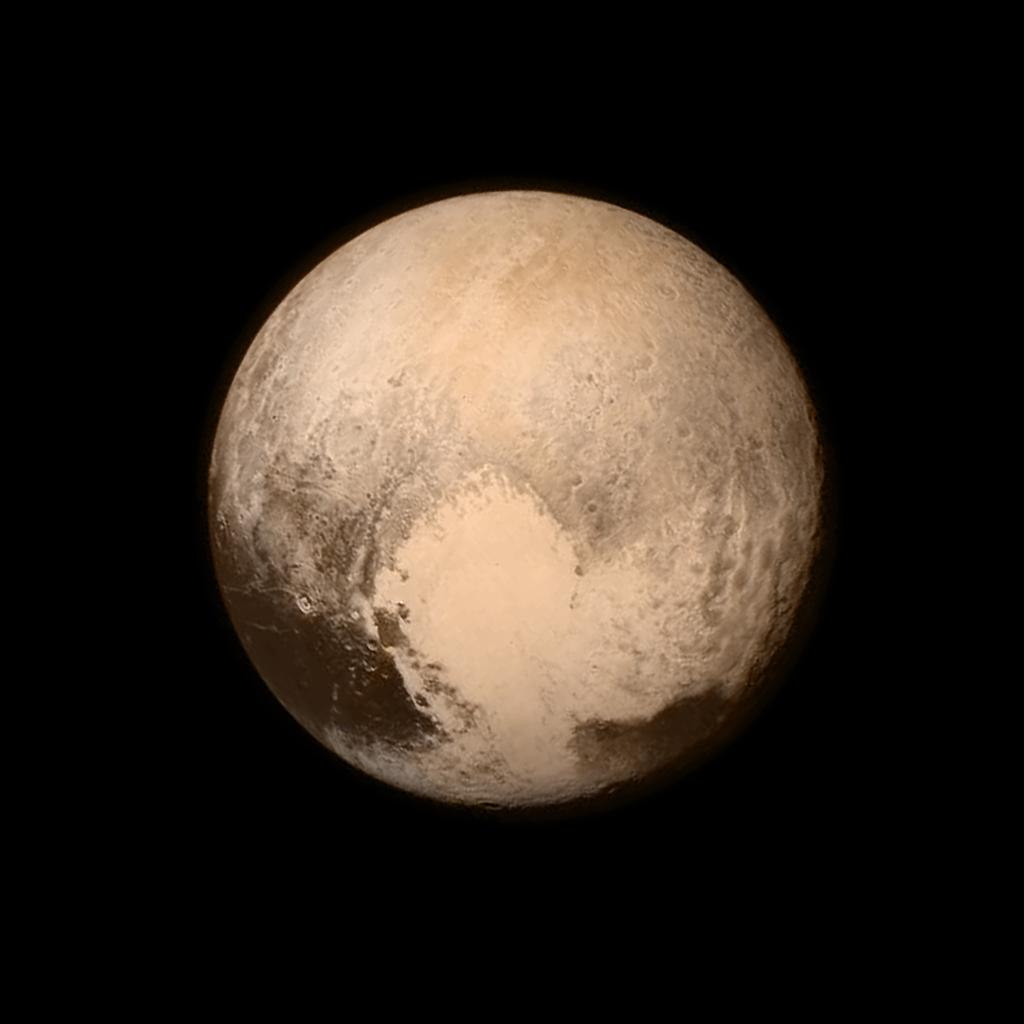
\includegraphics[width=0.5\textwidth]{figures/PIA19708-orig.jpg}
\caption[Shot description of the figure 1.1.]{Long description of figure 1 (Pluto captured by New Horizons). Note: there is a short description which will show on your list of figures. Image taken from \url{https://images-assets.nasa.gov/image/PIA19708/PIA19708~orig.jpg}.}
\label{fig1}
\end{figure*}

\subsection{One Horizontal Figure}
Figure~\ref{fig2} is an example of landscape image, which is Ultima Thule captured by New Horizons extended mission.


\begin{landscape}
\begin{figure*}[htb!]
\center
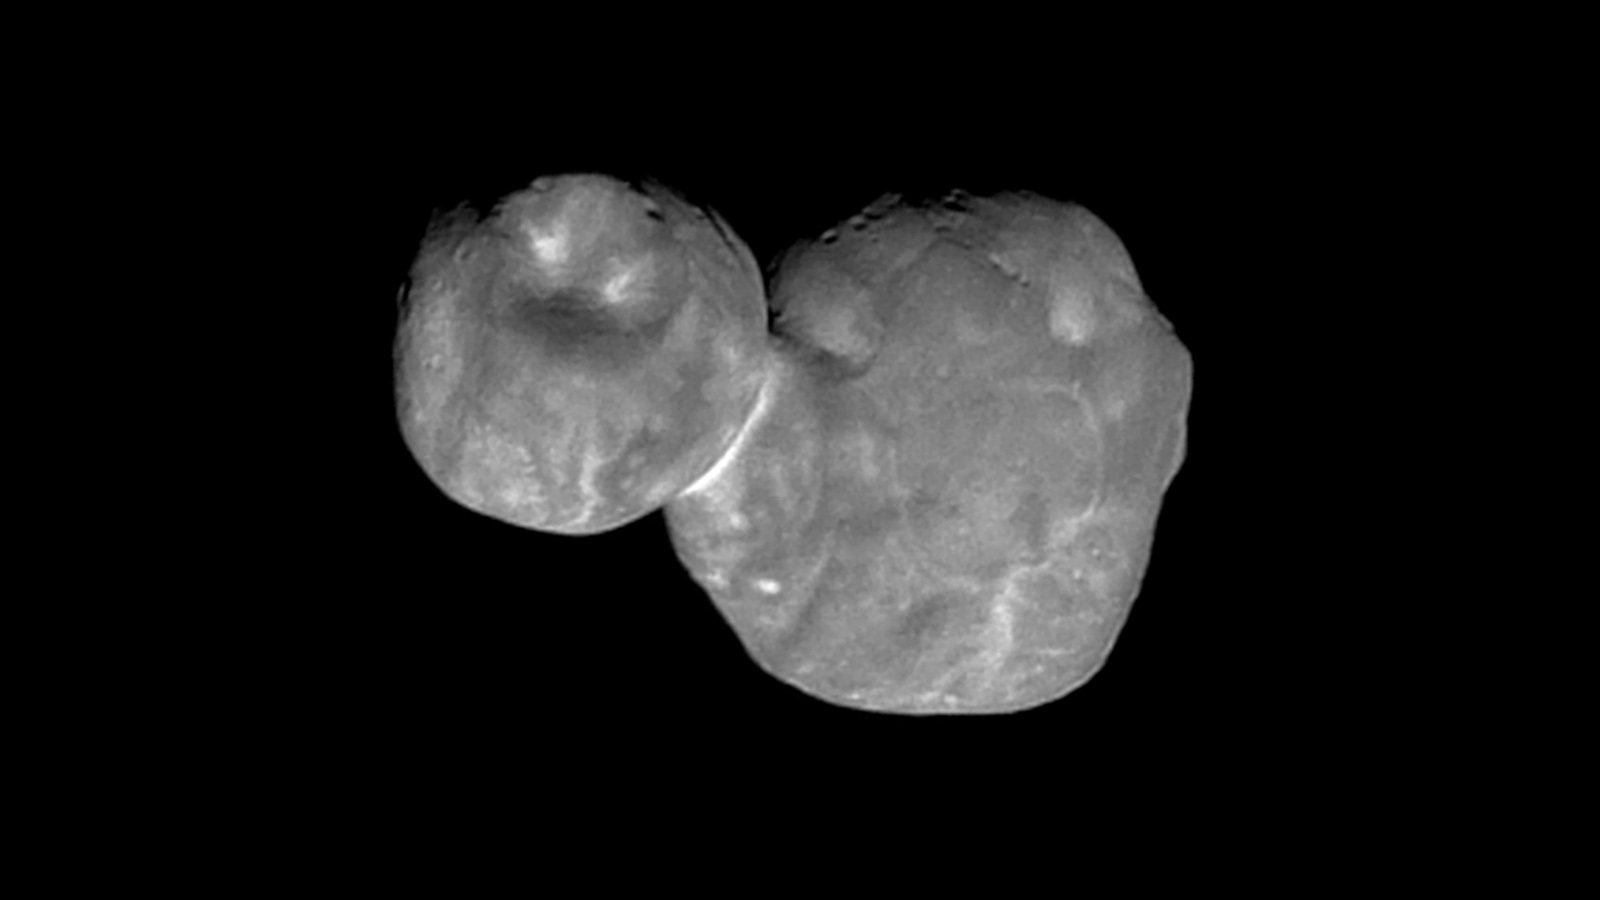
\includegraphics[width=\linewidth]{figures/819_MU69_1600.jpg}
\caption[Shot description of the figure 1.2.]{Long description of figure 1.2 (Ultima Thule captured by New Horizons). Note: there is a short description which will show on your list of figures. Note: in the  \textbackslash{includegraphics} command, use \textbackslash{linewidth} instead of \textbackslash{textwidth} to occupy almost the entire field of view. Image taken from \url{https://solarsystem.nasa.gov/system/news_items/main_images/819_MU69_1600.jpg}.}
\label{fig2}
\end{figure*}
\end{landscape}

\subsection{A Set of Subfigures}
Figure~\ref{fig3} is an example of a set of subfigures. You can cite the panels individually: Figure~\ref{fig3-a}, Figure~\ref{fig3-b}, and Figure~\ref{fig3-c}.


\begin{figure*}[htb!]
\center
\begin{subfigure}{0.67\linewidth}
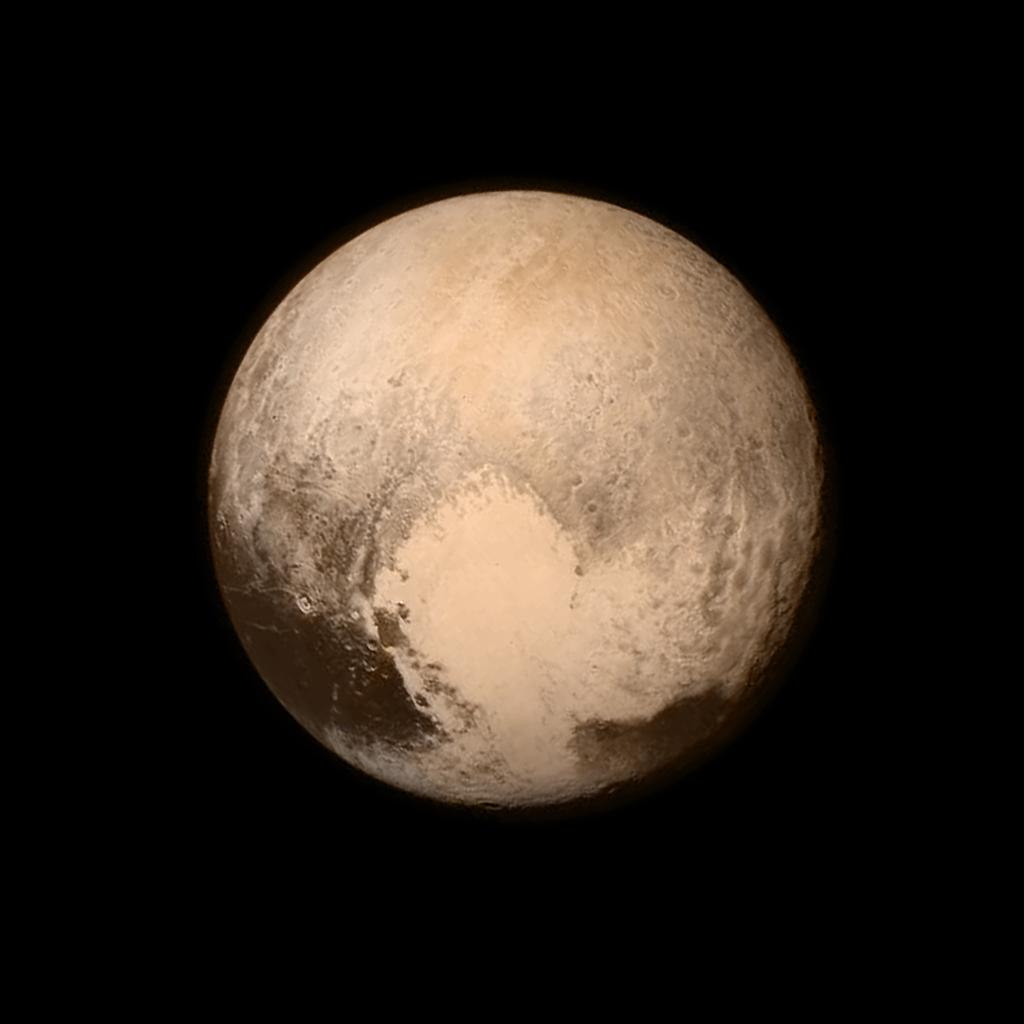
\includegraphics[width=\textwidth]{figures/PIA19708-orig.jpg}
\caption{Caption 1.}\label{fig3-a}
\end{subfigure}
\begin{subfigure}{0.35\linewidth}
\center
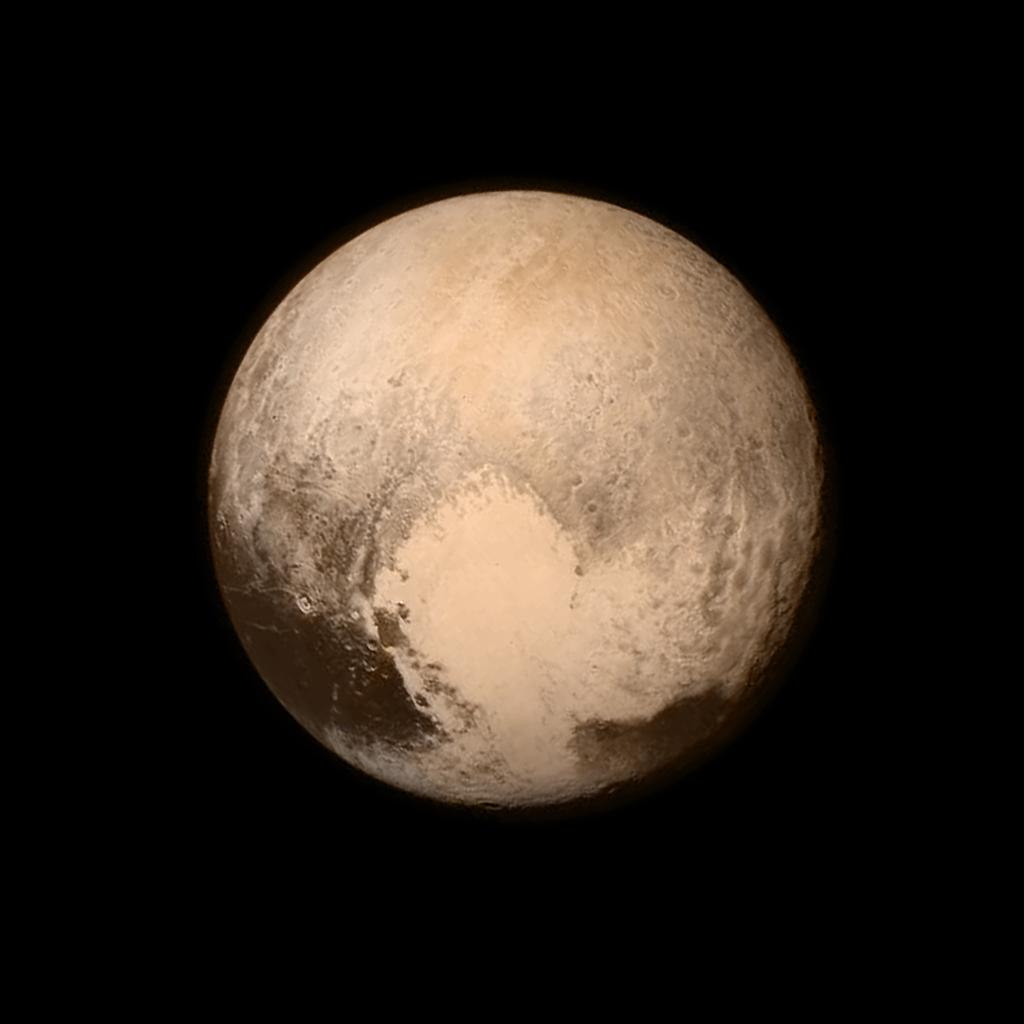
\includegraphics[width=\textwidth]{figures/PIA19708-orig.jpg}
\caption{Caption 2.}\label{fig3-b}
\end{subfigure}
\begin{subfigure}{0.24\linewidth}
\center
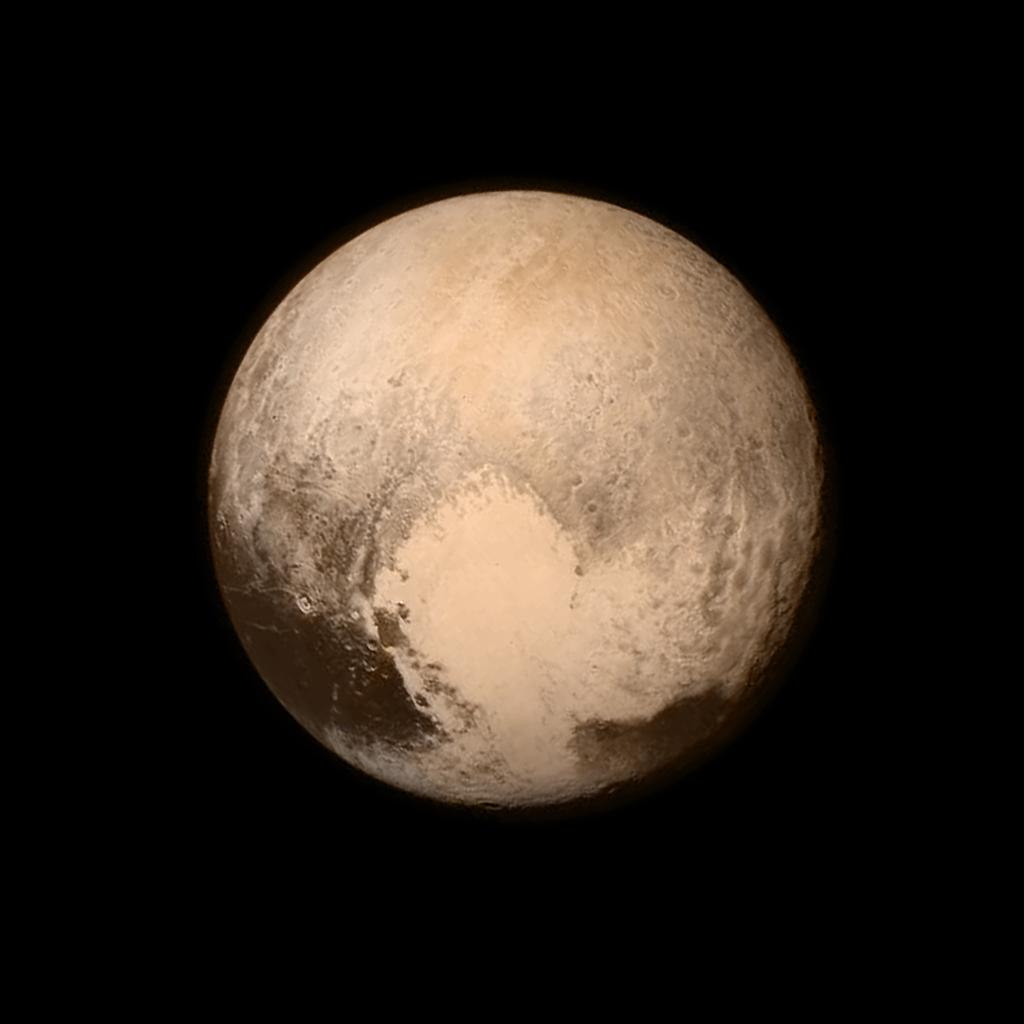
\includegraphics[width=\textwidth]{figures/PIA19708-orig.jpg}
\caption{Caption 3.}\label{fig3-c}
\end{subfigure}
\caption[Short description of figure 1.3.]{Long description of figure 1.3.}\label{fig3}
\end{figure*}
\section{Citing Chapters}
Chapter~\ref{chapter-apj} has the citations in the Astrophysical Journal\footnote{\url{https://iopscience.iop.org/journal/0004-637X}} (ApJ) style, it also shows how to use a long table. Chapter~\ref{chapter-apj-dup} has a normal table.

\cleardoublepage
\printbibliography[title={References}]
\end{refsection}

\begin{refsection}[chapter_apj/apj_chapter.bib]
\chapter{Chapter with Citation in ApJ Style}\label{chapter-apj}
\paragraph*{Abstract} Put your abstract in.
\section{Citation Examples}
You can cite a reference using \textbackslash{citet\{\}}, \textbackslash{citep\{\}}, and \textbackslash{citealp\{\}}. They will look like this:

\citet{ren18}, 

\citep{ren18},

and \citealp{ren18}.

You can just copy the AAS bibtex entires from ADS\footnote{\url{https://ui.adsabs.harvard.edu}}, and paste them in the .bib file.

\section{Equation and Table Examples}\label{sec:alpha}
This is your section alpha. 
\subsection{Equation}\label{eq-sample}
This is an equation sample taken from \citet{ren18}:
\begin{equation}
T_{\text{NMF}} = D_{\text{NMF}} + S_{\text{NMF}},\label{eq-example}
\end{equation}
where the subscript ${}_{\text{NMF}}$ means performing the NMF modeling result for the stellar signal ($S$) or disk signal ($D$) alone.

You can refer to the equation as Equation~\eqref{eq-example}.

\subsection{Long Table}\label{appendixSymbols}
Table~\ref{tab:nmf-sym} is part of a long table that was previous presented in an ApJ paper \citep{ren18}. The format was changed from the deluxetable style in ApJ.

{
\fontsize{10}{12}
\begin{center}
\begin{longtable}{cp{2cm}cp{6cm}}
\caption[Short table description 1.]{Long description of table 1}\label{tab:nmf-sym}\\
\hline\hline
Symbol	&	Expression 	& Dimension	& Meaning \\
\hline
\endfirsthead
\multicolumn{4}{l}{\sl \tablename\ \thetable{} -- (continued)} \\
\hline\hline
Symbol	&	Expression 	& Dimension	& Meaning \\
\hline
\endhead
\hline
{\sl (continued)} \\
\endfoot
\hline

\endlastfoot
$\circ$ & $(A\circ B)_{ij} = A_{ij}B_{ij}$ & & Element-wise (Hadamard) multiplication for matrices $A$ and $B$ of same dimension.\\
$D$ & & $1\times N_{\text{pix}}$ & Flattened image of the astrophysical signal (i.e., no stellar information).\\
$\hat{D}$ & $T - \hat{f}T_{\text{NMF}}$& $1\times N_{\text{pix}}$ & Reduced best image of the astrophysical signal ($D$), obtained from BFF procedure.\\
$D_f$ & $T - fT_{\text{NMF}}$& $1\times N_{\text{pix}}$ & Reduced image of the astrophysical signal with scaling factor $f$.\\
$D_{\text{NMF}}$& $\omega^{({D})} H$& $1\times N_{\text{pix}}$ & NMF model of the astrophysical signal ($D$).\\
$\delta(\cdot)$ & &  & The change of the $(\cdot)$ item after one iteration.\\
$F_{\mathrm{disk}}/F_{\mathrm{star}}$ & & & Flux ratio between the disk and the star.\\
$f$ & &  & Scaling factor, where $0 < f < 1$.\\
$\hat{f}$ & &  & Optimum scaling factor obtained from the BFF procedure, corresponding with $\hat{D}$.\\
$H$, $H^{(k)}$, $H^{(k+1)}$ & $[H_1^{T}, \cdots, H_n^T]^T$ & $n \times N_{\text{pix}}$ & NMF component matrix for the reference cube.\\
$H_1$, $H_i$, $H_n$ &  & $ 1 \times N_{\text{pix}}$ & The $1$-st, $i$-th, and $n$-th NMF component for the reference cube ($R$).\\
${(\cdot)}^{(k)}$, ${(\cdot)}^{(k+1)}$ & superscript &  & Iteration step number.\\
$\mu_f^{(k)}$ & & & The median of the pixels in $D_f$ at iteration step $k$.\\
$N_{\text{pix}}$& &  & Number of pixels in each image.\\
$N_{\text{ref}}$& &  & Number of images in the reference cube ($R$).\\
\end{longtable}
\end{center}}
The above table crosses different pages automatically. If you find a way to use the deluxetable directly, please do not use this format since it takes a few minutes to do the conversion.

\newpage
\section{Appendix}
This is your appendix for this chapter.
\cleardoublepage
\printbibliography[title={References}]
\end{refsection}


\begin{refsection}[chapter_apj_dup/apj_dup_chapter.bib]
\chapter{Another Chapter in \textit{ApJ} Style}\label{chapter-apj-dup}
%%%%%%%%%%%%%%%%%%%%%%%%%%%%%%%%%%%%%%%%%%%%%%%%%%%%%%%%%%%%%
Note: if you want italic font in your chapter title, use \textbackslash{textit}\{\} rather than \textbackslash{it}\{\} to have a better formatting in the Table of Contents.
\paragraph*{Abstract} This is your abstract.

\section{Table example}
Table~\ref{tab:stis-obs} has been presented in \citet{ren17}. It is not presented in \citet{ren18}. I am citing two references just to show you that the Reference section for this table will have two entries.

In the .bib file, you do not have to arrange the entries by their citation order! And you can add more entries---they will \textbf{not} appear on the References section as long as you don't cite them.


\begin{table}[htb!]
\centering
\caption[Short table description 2.]{Long table description 2.}
\label{tab:stis-obs}
\begin{tabular}{ccc}\hline\hline
   & Proposed Aperture Name & Number of Flat-Fielded Files \\ \hline
1  & BAR10                  & 116             \\
2  & {\bf WEDGE A0.6}             & {\bf 228}            \\
3  & {\bf WEDGE A1.0}             & {\bf 493}             \\
4  & WEDGE A1.8             & 86              \\
5  & WEDGE A2.0             & 39              \\
6  & WEDGE A2.5             & 1               \\
7  & WEDGE A2.8             & 5               \\
8  & WEDGE B1.0             & 37              \\
9  & WEDGE B1.8             & 8               \\
10 & WEDGE B2.0             & 9               \\
11 & WEDGE B2.5             & 116             \\
12 & WEDGE B2.8             & 5\\ \hline
\end{tabular}
\end{table}

\cleardoublepage
\printbibliography[title={References}]
\end{refsection}


%\begin{refsection}[chapterNMF/nmf_chapter.bib] % put your own chapter here in this format
%\include{chapterNMF/nmf_chapter}
%\cleardoublepage
%\printbibliography[title={References}]
%\end{refsection}

\begin{refsection}[conclusion_chapter/conclusion_chapter.bib]
\chapter{Conclusion}
\label{chap:conclusion}
\section{Results}
Blah blah blah. Blah blah blah. Blah blah blah.

\section{Ongoing Work and Future Exploration}
\paragraph*{Tackling Some Exciting Problems}

Blah blah blah.

\textit{Methodology}: Blah blah blah.
    
\textit{Expected Results}: Blah blah blah.
\cleardoublepage
\printbibliography[title={References}]
\end{refsection}


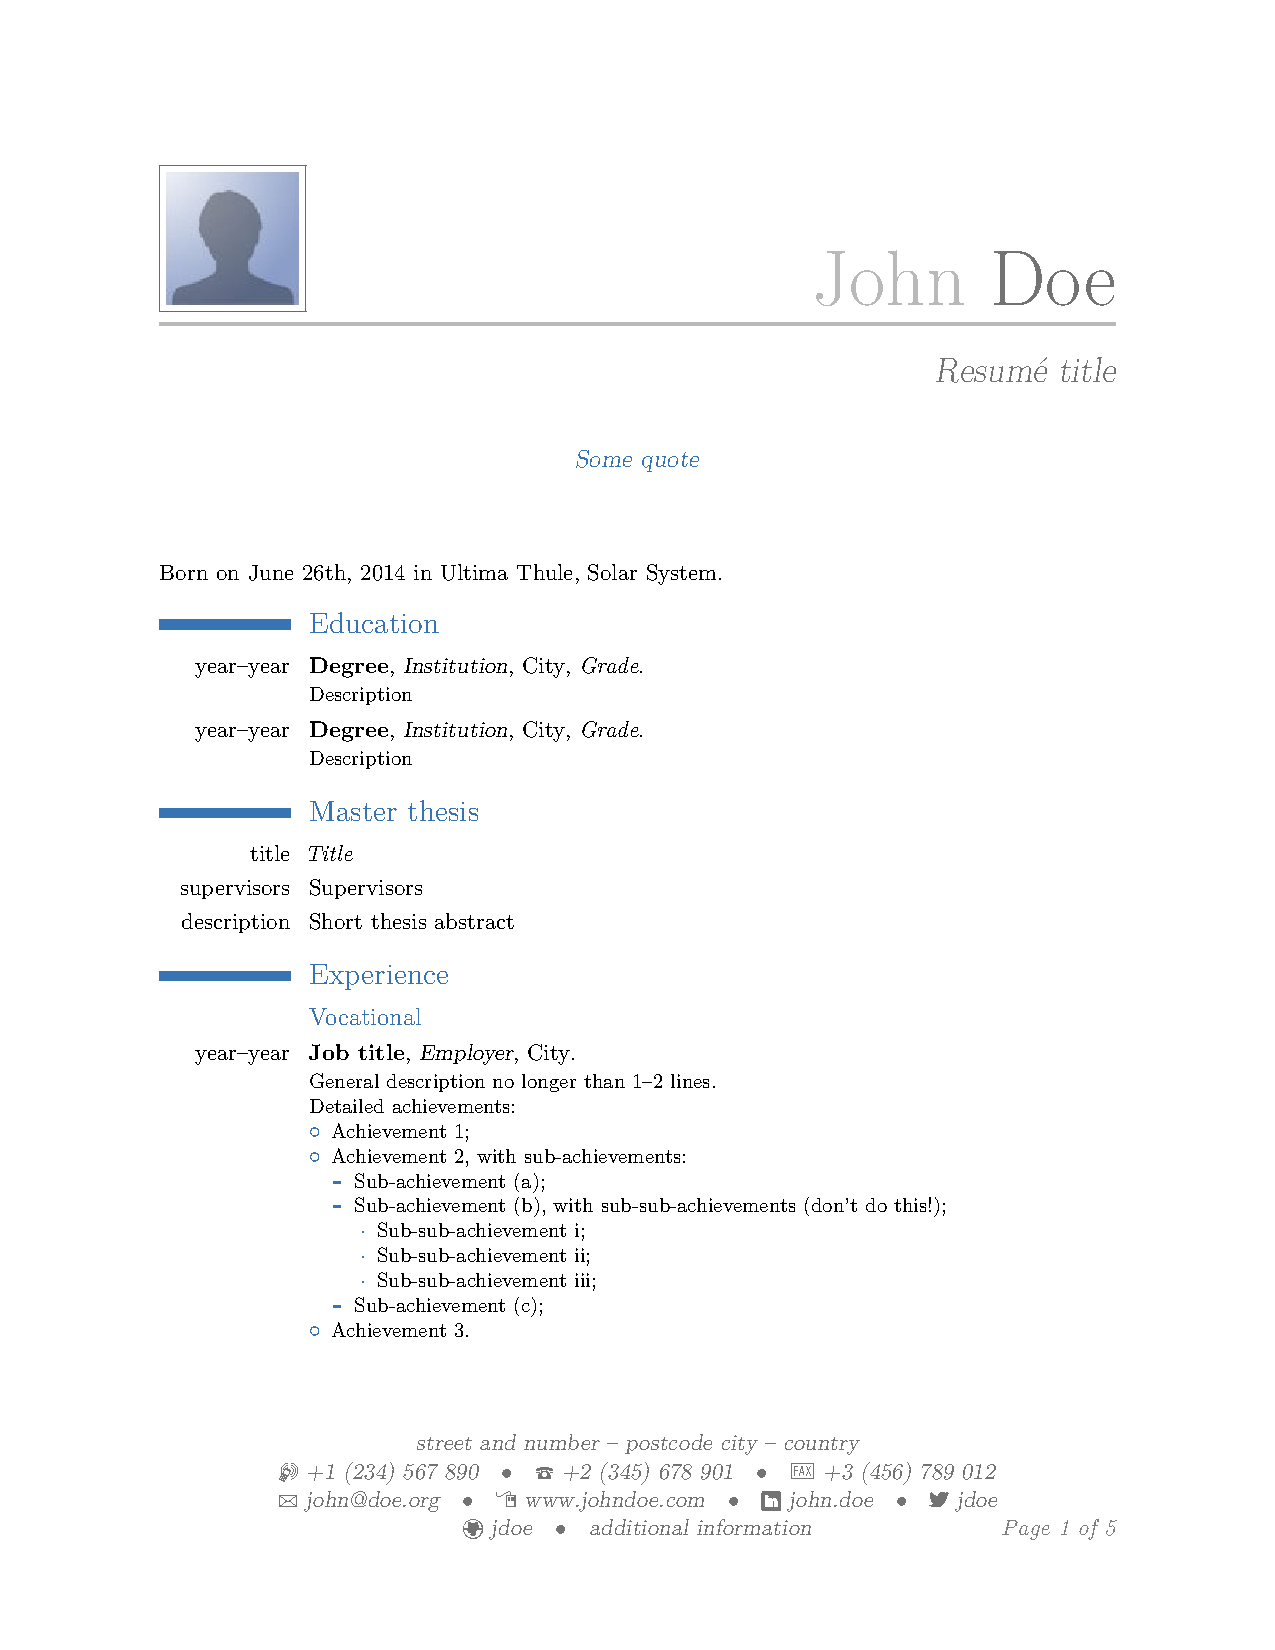
\includepdf[pages={-}, pagecommand={\thispagestyle{plain}}]{moderncv/template-cv.pdf}
% You can also use your cv in your style.
% If you are using the moderncv template, please compile the cv first (added by Bin Ren)

\end{CJK*} % Ending simplified Chinese characters (added by Bin Ren)
\end{document}
